%%%%%%%%%%%%%%%%%%%%%%%%%%%%%%%%%%%%%%%%%
% baposter Landscape Poster
% LaTeX Template
% Version 1.0 (11/06/13)
%
% baposter Class Created by:
% Brian Amberg (baposter@brian-amberg.de)
%
% This template has been downloaded from:
% http://www.LaTeXTemplates.com
%
% License:
% CC BY-NC-SA 3.0 (http://creativecommons.org/licenses/by-nc-sa/3.0/)
%
%%%%%%%%%%%%%%%%%%%%%%%%%%%%%%%%%%%%%%%%%

%----------------------------------------------------------------------------------------
%	PACKAGES AND OTHER DOCUMENT CONFIGURATIONS
%----------------------------------------------------------------------------------------

% Dimensions of 48 x 27 projects full screen on my computer in such a way as to fill the screen.  It will also print out 4' wide, so can be used in a virtual and physical case.
\documentclass[landscape,paperwidth=40in,paperheight=30in,fontscale=0.32]{baposter} % Adjust the font scale/size here

\usepackage{graphicx} % Required for including images
\graphicspath{{figures/}} % Directory in which figures are stored

\usepackage{amsmath} % For typesetting math
\usepackage{amssymb} % Adds new symbols to be used in math mode

\usepackage{booktabs} % Top and bottom rules for tables
\usepackage{enumitem} % Used to reduce itemize/enumerate spacing
%\usepackage{palatino} % Use the Palatino font
\usepackage{palatino} % Use the Helvetica font
\usepackage[font=small,labelfont=bf]{caption} % Required for specifying captions to tables and figures

\usepackage{multicol} % Required for multiple columns
\setlength{\columnsep}{1.5em} % Slightly increase the space between columns
\setlength{\columnseprule}{0mm} % No horizontal rule between columns
\usepackage{vwcol}

\usepackage{tikz} % Required for flow chart
\usetikzlibrary{shapes,arrows} % Tikz libraries required for the flow chart in the template

\newcommand{\compresslist}{ % Define a command to reduce spacing within itemize/enumerate environments, this is used right after \begin{itemize} or \begin{enumerate}
\setlength{\itemsep}{1pt}
\setlength{\parskip}{0pt}
\setlength{\parsep}{0pt}
}

\definecolor{lightblue}{rgb}{0.145,0.6666,1} % Defines the color used for content box headers


\begin{document}

\begin{poster}
{
columns=3,  %override the default number of columns
headerborder=closed, % Adds a border around the header of content boxes
colspacing=1em, % Column spacing
bgColorOne=white, % Background color for the gradient on the left side of the poster
bgColorTwo=white, % Background color for the gradient on the right side of the poster
borderColor=lightblue, % Border color
headerColorOne=black, % Background color for the header in the content boxes (left side)
headerColorTwo=lightblue, % Background color for the header in the content boxes (right side)
headerFontColor=white, % Text color for the header text in the content boxes
boxColorOne=white, % Background color of the content boxes
textborder=roundedleft, % Format of the border around content boxes, can be: none, bars, coils, triangles, rectangle, rounded, roundedsmall, roundedright or faded
eyecatcher=false, % Set to false for ignoring the left logo in the title and move the title left
headerheight=0.125\textheight, % Height of the header
headershape=roundedright, % Specify the rounded corner in the content box headers, can be: rectangle, small-rounded, roundedright, roundedleft or rounded
headerfont=\Large\bf\textsc, % Large, bold and sans serif font in the headers of content boxes
%textfont={\setlength{\parindent}{1.5em}}, % Uncomment for paragraph indentation
linewidth=2pt % Width of the border lines around content boxes
}
%----------------------------------------------------------------------------------------
%	TITLE SECTION
%----------------------------------------------------------------------------------------
%

{\bf\textsc{Introduction to Machine Learning in the Physical Sciences: \\Student Experiences}\vspace{0.25em}} % Poster title
{\textsc{Simon J. L. Billinge$^1$, Sanat Kumar$^2$, Sarah Alsharif$^1$, Candice Chiu$^4$, Joshua Crawford$^2$, Elizabeth Katzman$^2$, Alperen Koc$^3$, Tymon Nieduzak$^3$, Benjamin Schwartz$^2$, Zoe Zachko$^1$, Tieqiong Zhang$^1$, Grant Zhou$^3$\\%\hspace{12pt}
$^1$Applied Physics and Applied Mathematics, $^2$Chemical Engineering, $^3$Civil Engineering, $^4$Biomedical Engineering}} % Author names and institution
{
\includegraphics[height=6em]{figures/seas_logo.png}\hspace{0pt}} % Second university/lab logo on the right


%%%%%%%%%%%%%%%%%%%%%%%%%%%%%%%%%%%%%%%%%%%%%%%%%%%%%%%%%%%%%%%%%%%%%
\headerbox{Overview and Motivation}{name=row1fixer,column=0,row=0,span=1}{

\begin{multicols}{2}

\textbf{What}: A one-semester accelerated machine learning (ML) course applied to STEM research problems.
\vskip 2pt

\textbf{Participants}: graduate students and physical science undergraduates interested in applying ML to their research, this semesters cohort is a mix of Materials Science, Chemical, Biomedical, and Civil Engineering. 
\vskip 2pt

\textbf{Motivation}: Building an understanding of machine learning through interaction with Edexes, then applying these new skills to research projects in each students respective disciplines. 
\vskip 2pt

\textbf{Scope}: unsupervised and supervised learning, decision trees, logistic regression, neural nets, etc., applied to physical science research problems
\vskip 2pt

\textbf{Prerequisites}: Physical science knowledge and basic programming. Prior ML knowledge is NOT required.

\end{multicols}

\vskip 5pt
}
%%%%%%%%%%%%%%%%%%%%%%%%%%%%%%%%%%%%%%%%%%%%%%%%%%%%%%%%%%%%%%%%%%%%%
\headerbox{Learning Materials: EdEx's}{name=introduction,column=1,row=0,span=1, bottomaligned=row1fixer}
{

%\vspace{-2em}

\begin{multicols}{2}

\textbf{What:} EdEx stand for educational examples. They are hands-on tutorials designed to walk students through machine-learning applications from published research. 
\vskip 3pt

\textbf{EdExes:} 
\begin{itemize}[leftmargin=10pt, itemsep=2pt]
    \item integrate with the theoretical lecture component of the course
    \item based on published research conducted primarily here at Columbia Engineering
    \item Students work together in pairs or teams to solve the given problem. We are working primarily in Jupyter Notebooks. At the end of each Edex, one group is chosen to present their work to the class. 
\end{itemize}

\textbf{Tools introduced}: Jupyter notebooks, conda, git, scikit-learn, keras, tensorFlow.

\end{multicols}

}

%%%%%%%%%%%%%%%%%%%%%%%%%%%%%%%%%%%%%%%%%%%%%%%%%%%%%%%%%%%%%%%%%%%%%
\headerbox{Status and team}{name=introduction3,column=2,row=0,span=1,bottomaligned=row1fixer}{
\textbf{Status}: the course is currently being taken by 10 students and is under development as MSAE4990.\\
\vspace{-10pt}
\textbf{Funded by}:
\begin{center}
    
\includegraphics[width=0.55\linewidth]{figures/collab_logo.png}
\end{center}
\vspace{-10pt}


\begin{center}
    \textbf{The Students}: The students are a mix of Masters candidates, PHD candidates and undergraduate students across four different disciplines. The three primary research areas are EV safety, batteries, and ligament repair. The class is primarily discussion based. We are enthusiastic about sharing our individual passions and improving our problem solving capabilities so we can all be more effective communicators and engineers. 

\end{center} 

}

%%%%%%%%%%%%%%%%%%%%%%%%%%%%%%%%%%%%%%%%%%%%%%%%%%%%%%%%%%%%%%%%%%%%%
\headerbox{Class Outcomes}{name=row2fixer,column=2,row=1,below=row1fixer}{

{}
\begin{multicols}{2}

\textbf{Adapting Course Materials}: Students are currently working on developing new Edexes, as well as providing feedback on the course. The new Edexes are being developed to acknowledge problems that have arisen as we learn about ML. These new Edexes help streamline the class experience and add to its impact. Some examples of new material are unit testing and package development.   
\vskip 3pt

\textbf{ML Solutions to Research}: Students present their active research. Currently, we are brainstorming ML solutions to some of the obstacles in the projects. We will then narrow down which problem to investigate further. The goal is to work together as a class to apply our new found knowledge from the Edexes to a relevant problem and publish a paper. 
\vskip 3pt

\textbf{Further Machine Learning Knowledge}: Throughout the rest of the term, we plan to expand our ML skill set, and continue to apply it to Materials Science problems. An upcoming Edex is focused on membrane permeability for individual gas separation. This will teach us about permutation importance and Shapley Values.  

\textbf{Community Focus}: This class encourages open collaboration between disciplines, through extensive classroom participation and interaction with the larger ML community online. This is a course designed to be accessible and engaging for anyone interested in learning a new problem solving framework. 
\vskip 3pt

\vskip 0.5em

\end{multicols}
}

%%%%%%%%%%%%%%%%%%%%%%%%%%%%%%%%%%%%%%%%%%%%%%%%%%%%%%%%%%%%%%%%%%%%%
\headerbox{Edex 2: Space Group Classifier} {name=p21,column=1,span=1,row=1,below=row1fixer,bottomaligned=row2fixer%,above=row3
}
{
\begin{multicols}{2}
\begin{center}
    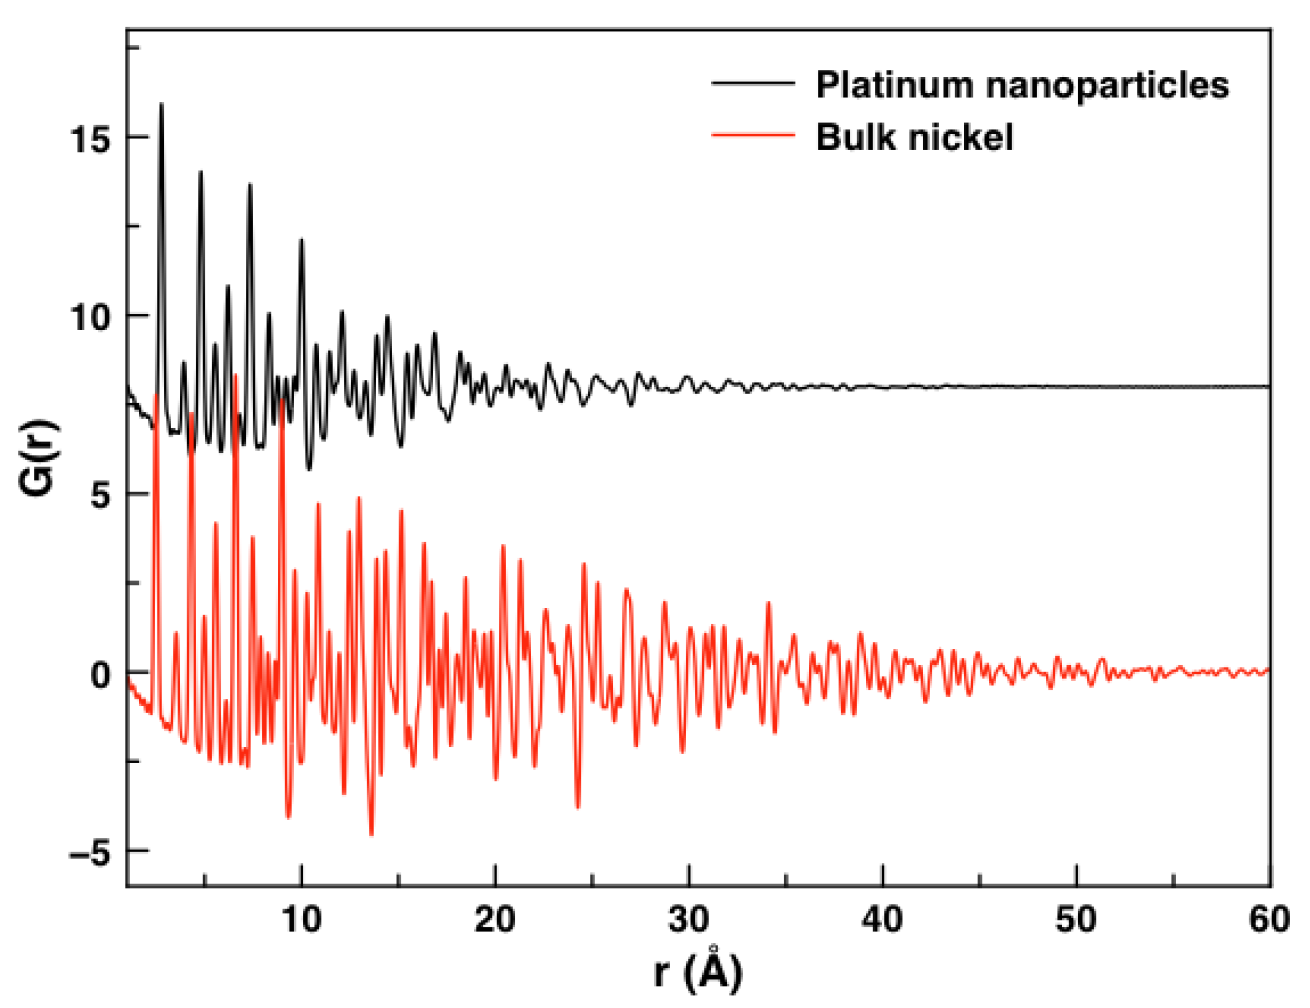
\includegraphics[width=1.0\linewidth]{figures/pdf.png}
    {\small Image source: Billinge Group}
\end{center}

\begin{center}
    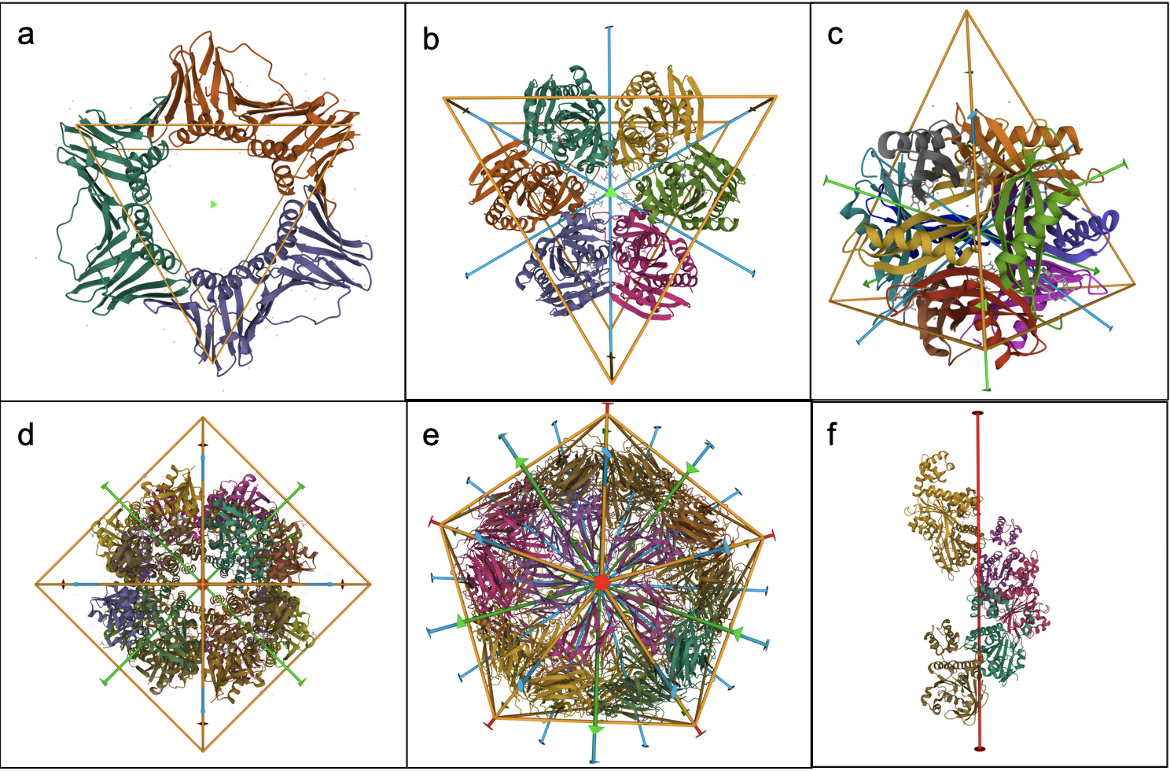
\includegraphics[width=1.0\linewidth]{figures/symmetry.png}
    {\small Image source: RCSB Protein Databank}
\end{center}

\textbf{Goal}: predict the space group (SG) of a crystal structure giving the measured atomic pair distribution function (PDF). 
 \vskip 3pt

\textbf{Problem}: SG encodes structural symmetries of atomic arrangements in a material. PDF is an x-ray measurement of the material. There is no direct way of getting SG from the PDF.

\textbf{Motivation}: The ML model can quickly predict the most likely space groups and give insights into the structure-property relationships.
 \vskip 3pt

\textbf{Model}: convolutional neural networks.
\vskip 3pt

\textbf{Training}: 40,000 PDFs that are calculated from 8 of the most common space groups.

\vskip 0.5em
{\small
Liu, C. H., et al. Acta Crystallographica Section A: Foundations and Advances, 75(4), 633-643.
}
\end{multicols}

}

%%%%%%%%%%%%%%%%%%%%%%%%%%%%%%%%%%%%%%%%%%%%%%%%%%%%%%%%%%%%%%%%%%%%%
\headerbox{Edex 1: Predicting melting temps}{name=row2fixer,column=0,row=1,below=row1fixer}{

{}
\begin{center}
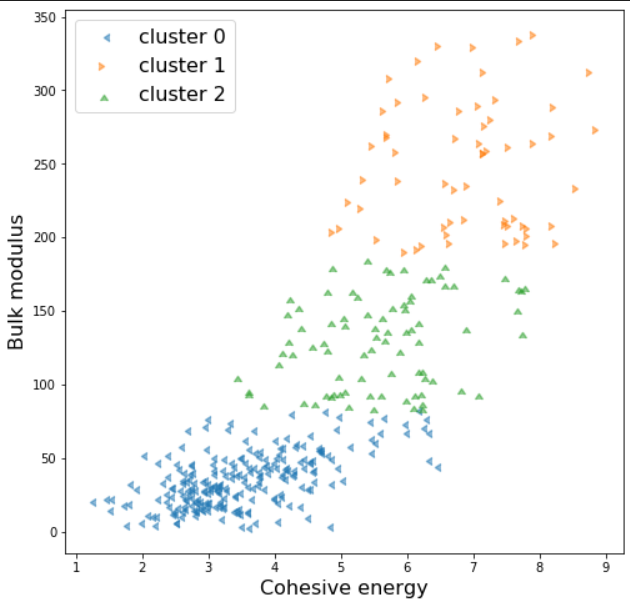
\includegraphics[width=0.55\linewidth]{figures/edex4.png}
\end{center}
\begin{multicols}{2}

\textbf{Goal}: Predict the melting temperature of inorganic materials given just the chemistry of the constituents. 
\vskip 3pt

\textbf{Problem}: We need quick and reliable low-cost predictions of melting temperature for metal extraction. Chemical variability means that one model does not work over high-variance data.
\vskip 3pt

\textbf{Student Experience}: A  variety of different methods were used, including different clustering methods and SVR in an attempt to boost performance. 

\textbf{Model}: k-Means clustering, various other clustering and regression models implemented via scikit-learn
\vskip 3pt

\vskip 0.5em
{\small Gharakhanyan, V., Urban, A., In preparation (2023).}

\end{multicols}
}





\end{poster}


\end{document}


%----------------------------------------------------------------------------------------
%	RESULTS 1
%----------------------------------------------------------------------------------------

\headerbox{Results 1}{name=results,column=2,span=2,row=0}{

\begin{multicols}{2}
\vspace{1em}
\begin{center}
\includegraphics[width=0.8\linewidth]{placeholder}
\captionof{figure}{Figure caption}
\end{center}

Aliquam auctor, metus id ultrices porta, risus enim cursus sapien, quis iaculis sapien tortor sed odio. Mauris ante orci, euismod vitae tincidunt eu, porta ut neque. Aenean sapien est, viverra vel lacinia nec, venenatis eu nulla. Maecenas ut nunc nibh, et tempus libero. Aenean vitae risus ante. Pellentesque condimentum dui. Etiam sagittis purus non tellus tempor volutpat. Donec et dui non massa tristique adipiscing.
\end{multicols}

%------------------------------------------------

\begin{multicols}{2}
\vspace{1em}
Sed fringilla tempus hendrerit. Vestibulum ante ipsum primis in faucibus orci luctus et ultrices posuere cubilia Curae; Etiam ut elit sit amet metus lobortis consequat sit amet in libero. Lorem ipsum dolor sit amet, consectetur adipiscing elit. Phasellus vel sem magna. Nunc at convallis urna. isus ante. Pellentesque condimentum dui. Etiam sagittis purus non tellus tempor volutpat. Donec et dui non massa tristique adipiscing. Quisque vestibulum eros eu.

\begin{center}
\includegraphics[width=0.8\linewidth]{placeholder}
\captionof{figure}{Figure caption}
\end{center}

\end{multicols}
}


%------------------------------------------------

%----------------------------------------------------------------------------------------
%	MATERIALS AND METHODS
%----------------------------------------------------------------------------------------

\headerbox{Materials \& Methods}{name=method,column=0,below=objectives,bottomaligned=conclusion}{ % This block's bottom aligns with the bottom of the conclusion block

The following materials were required to complete the research:

\begin{itemize}\compresslist
\item Curabitur pellentesque dignissim
\item Eu facilisis est tempus quis
\item Duis porta consequat lorem
\item Eu facilisis est tempus quis
\end{itemize}

The following equations were used for statistical analysis:

\begin{equation}
\cos^3 \theta =\frac{1}{4}\cos\theta+\frac{3}{4}\cos 3\theta
\label{eq:refname}
\end{equation}\

\begin{equation}
E = mc^{2}
\label{eqn:Einstein}
\end{equation}

Phasellus imperdiet, tortor vitae congue bibendum, felis enim sagittis lorem, et volutpat ante orci sagittis mi. Morbi rutrum laoreet semper. Morbi accumsan enim nec tortor consectetur non commodo nisi sollicitudin. Proin sollicitudin. Pellentesque eget orci eros. Fusce ultricies, tellus et pellentesque fringilla, ante massa luctus libero, quis tristique purus urna nec nibh.
}

%----------------------------------------------------------------------------------------
%	RESULTS 2
%----------------------------------------------------------------------------------------

\headerbox{Results 2}{name=results2,column=1,below=objectives,bottomaligned=conclusion}{ % This block's bottom aligns with the bottom of the conclusion block

Donec faucibus purus at tortor egestas eu fermentum dolor facilisis. Maecenas tempor dui eu neque fringilla rutrum. Mauris \emph{lobortis} nisl accumsan.

\begin{center}
\begin{tabular}{l l l}
\toprule
\textbf{Treatments} & \textbf{Response 1} & \textbf{Response 2}\\
\midrule
Treatment 1 & 0.0003262 & 0.562 \\
Treatment 2 & 0.0015681 & 0.910 \\
Treatment 3 & 0.0009271 & 0.296 \\
\bottomrule
\end{tabular}
\captionof{table}{Table caption}
\end{center}

Nulla ut porttitor enim. Suspendisse venenatis dui eget eros gravida tempor. Mauris feugiat elit et augue placerat ultrices. Morbi accumsan enim nec tortor consectetur non commodo.

\begin{center}
\begin{tabular}{l l l}
\toprule
\textbf{Treatments} & \textbf{Response 1} & \textbf{Response 2}\\
\midrule
Treatment 1 & 0.0003262 & 0.562 \\
Treatment 2 & 0.0015681 & 0.910 \\
Treatment 3 & 0.0009271 & 0.296 \\
\bottomrule
\end{tabular}
\captionof{table}{Table caption}
\end{center}
}
%----------------------------------------------------------------------------------------
%	FUTURE RESEARCH
%----------------------------------------------------------------------------------------

\headerbox{Future Research}{name=futureresearch,column=1,span=2,aligned=references,above=bottom}{ % This block is as tall as the references block

\begin{multicols}{2}
Integer sed lectus vel mauris euismod suscipit. Praesent a est a est ultricies pellentesque. Donec tincidunt, nunc in feugiat varius, lectus lectus auctor lorem, egestas molestie risus erat ut nibh.

Maecenas viverra ligula a risus blandit vel tincidunt est adipiscing. Suspendisse mollis iaculis sem, in \emph{imperdiet} orci porta vitae. Quisque id dui sed ante sollicitudin sagittis.
\end{multicols}
}

%----------------------------------------------------------------------------------------
%	CONTACT INFORMATION
%----------------------------------------------------------------------------------------

\headerbox{Contact Information}{name=contact,column=3,aligned=references,above=bottom}{ % This block is as tall as the references block

\begin{description}\compresslist
\item[Web] www.university.edu/smithlab
\item[Email] john@smith.com
\item[Phone] +1 (000) 111 1111
\end{description}
}


%----------------------------------------------------------------------------------------
%----------------------------------------------------------------------------------------
%	REFERENCES
%----------------------------------------------------------------------------------------

\headerbox{References}{name=references,column=0,above=bottom}{

\renewcommand{\section}[2]{\vskip 0.05em} % Get rid of the default "References" section title
\nocite{*} % Insert publications even if they are not cited in the poster
\small{ % Reduce the font size in this block
\bibliographystyle{unsrt}
\bibliography{sample} % Use sample.bib as the bibliography file
}}

\begin{multicols}{2}

\tikzstyle{decision} = [diamond, draw, fill=blue!20, text width=4.5em, text badly centered, node distance=2cm, inner sep=0pt]
\tikzstyle{block} = [rectangle, draw, fill=blue!20, text width=5em, text centered, rounded corners, minimum height=4em]
\tikzstyle{line} = [draw, -latex']
\tikzstyle{cloud} = [draw, ellipse, fill=red!20, node distance=3cm, minimum height=2em]

\begin{tikzpicture}[node distance = 2cm, auto]
\node [block] (init) {Initialize Model};
\node [cloud, left of=init] (Start) {Start};
\node [cloud, right of=init] (Start2) {Start Two};
\node [block, below of=init] (init2) {Initialize Two};
\node [decision, below of=init2] (End) {End};
\path [line] (init) -- (init2);
\path [line] (init2) -- (End);
\path [line, dashed] (Start) -- (init);
\path [line, dashed] (Start2) -- (init);
\path [line, dashed] (Start2) |- (init2);
\end{tikzpicture}

